\section{Summary}
Breast cancer is the second leading form of cancer among U.S women demanding further progress to accurately predict screening mammograms that have been found to reduce mortality. The advent of artificial intelligence in the bio-sciences has recently enabled radiologists to make better predictions through the support of deep learning based software. However, increasing the accuracy further is challenging due to two major obstacles: Firstly, the databases that provide the mammograms evolve quickly and can be very heterogeneous making the transfer to different databases difficult. Secondly, the tumors themselves only occupy a very small region of the image of the entire breast. Previous approaches that make use of annotated regions of interests (ROIs) struggle to transfer to databases that lack ROI annotations. For other methods that train their networks on the whole image it is hard to tell if they are acutally able to locate the clinically relevant lesions.
L. Shen et al. propose a method that targets both of these obstacles. They manage to leverage existing databases with ROI annotations while simultaneously maintaining the applicability to different datasets without these annotations. 
\newline
\newline
The presented model can be depicted as a two-step pipeline composed of the functions $f$ and $g$ in Figure \ref{fig1}.  The first segment consists of a patch classifier given by the 16-layer VGG netowrk (VGG16) or the 50-layer Resnet (Resnet 50) architecture which is pre-trained on patches of ROIs of mammorgraphies. These learned weights are then used as the weights of the convolutional filter for the whole input image resulting in a $u\times v$ grid of  probabilistic outputs for each of the $c$ classes, which is taken to be five:  benign calcification, malignant calcification, benign mass, malignant mass and background. $u,v$ depend on the ratio of the whole image to the ROI and the stride of the filter operation. 

\begin{figure}[H]
	\centering
	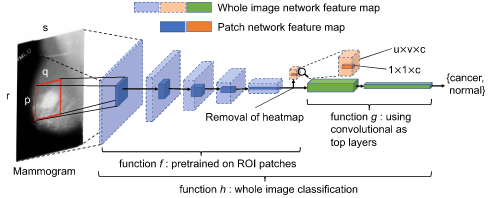
\includegraphics[width=0.7\textwidth]{ML1}
	\captionof{figure}{The pipeline structure of the model \cite{article}.}
	\label{fig1}
\end{figure}
\noindent The output of the patch classifier then serves as the input of two more blocks of convolutional layers (VGG or Resnet) followed by a global pooling layer. The idea is that these top layers 'scan' over the whole image receiving the classification of the individual patch by the first segment. These information are then pooled to produce a classification of the entire image. 
\newline 
\newline

\noindent
\begin{minipage}{0.5\textwidth}	
\noindent
The training and testing is performed on the datasets SBIS-DDSM and INbreast, of which the first one contains annotated ROIs and the second one doesn't to test the transferability of the model.
On the first dataset the training is divided into two parts beginning to train the patch classifier solely using sampled patches from the dataset. These patches are either part of the background or contain an ROI that belongs to one of the combined classes benign/malignant and calcification/mass. In the second step the entire network is trained using the whole images from the dataset.
\end{minipage}
\begin{minipage}[c]{0.5\textwidth}
	\centering
	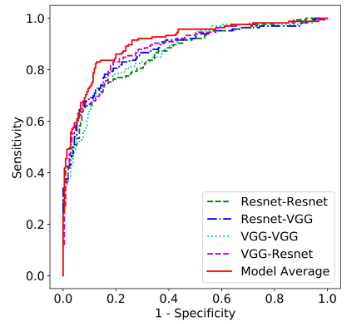
\includegraphics[width=1\textwidth]{ML2}
	%\captionof*{figure}{ ROC curve of the full model on the SBIS-DDSM dataset.}
	\label{fig2}		
\end{minipage}
The performance of the entire model for different configurations of Resnet and VGG is illustrated by the ROC curve achieving an AUC score of about 0.86. We see that none of the configurations is clearly superior to any of the other setups. 

ON INbreast the authors used the pre-trained patch classifier from the first dataset and merely trained the second part of the pipeline using entire images from INbreast. It turns out that the model achieves excellent performance with an average AUC score of 0.95 across different combinations of Resnet and VGG. Interestingly, already after 79 images the model reached AUC scores between 0.87 and 0.92. This suggests that the intensive part of training is fine-tuning the batch classifier to recognise shapes and textures of benign and malignant tissues. Adjusting the model to different intensity profiles of a specific dataset then requires much less data.
\newline
\newline
L. Shen et. al show that deep learning can be used to effectively predict screening mammographies. Their method is end-to-end learnable and applicable to different datasets once the batch classifier has been tuned. This enables a greater versatility since mammography systems evolve rapidly. However, labeled ROIs are still critical for the performance of the network and a lot of further improvement could rely on datasets containing more edge cases where errors still occur. 
